\documentclass[a4paper]{article}
\usepackage[spanish]{babel}
\usepackage[utf8]{inputenc}
\usepackage{charter}   % tipografia
\usepackage{graphicx}
%\usepackage{makeidx}
\usepackage{paralist} %itemize inline
\usepackage{algorithmicx}
\usepackage{algpseudocode}



%\usepackage{float}
%\usepackage{amsmath, amsthm, amssymb}
%\usepackage{amsfonts}
%\usepackage{sectsty}
%\usepackage{charter}
%\usepackage{wrapfig}
%\usepackage{listings}
%\lstset{language=C}


\usepackage{color} % para snipets de codigo coloreados
\usepackage{fancybox}  % para el sbox de los snipets de codigo

\definecolor{litegrey}{gray}{0.94}

% \newenvironment{sidebar}{%
% 	\begin{Sbox}\begin{minipage}{.85\textwidth}}%
% 	{\end{minipage}\end{Sbox}%
% 		\begin{center}\setlength{\fboxsep}{6pt}%
% 		\shadowbox{\TheSbox}\end{center}}
% \newenvironment{warning}{%
% 	\begin{Sbox}\begin{minipage}{.85\textwidth}\sffamily\lite\small\RaggedRight}%
% 	{\end{minipage}\end{Sbox}%
% 		\begin{center}\setlength{\fboxsep}{6pt}%
% 		\colorbox{litegrey}{\TheSbox}\end{center}}

\newenvironment{codesnippet}{%
	\begin{Sbox}\begin{minipage}{\textwidth}\sffamily\small}%
	{\end{minipage}\end{Sbox}%
		\begin{center}%
		\colorbox{litegrey}{\TheSbox}\end{center}}



\usepackage{fancyhdr}
\pagestyle{fancy}

%\renewcommand{\chaptermark}[1]{\markboth{#1}{}}
\renewcommand{\sectionmark}[1]{\markright{\thesection\ - #1}}

\fancyhf{}

\fancyhead[LO]{Sección \rightmark} % \thesection\ 
\fancyfoot[LO]{\small{Ángel Fernando More, Claudio Gomez, Fernando Otero}}
\fancyfoot[RO]{\thepage}
\renewcommand{\headrulewidth}{0.5pt}
\renewcommand{\footrulewidth}{0.5pt}
\setlength{\hoffset}{-0.8in}
\setlength{\textwidth}{16cm}
%\setlength{\hoffset}{-1.1cm}
%\setlength{\textwidth}{16cm}
\setlength{\headsep}{0.5cm}
\setlength{\textheight}{25cm}
\setlength{\voffset}{-0.7in}
\setlength{\headwidth}{\textwidth}
\setlength{\headheight}{13.1pt}

\renewcommand{\baselinestretch}{1.1}  % line spacing


% \setcounter{secnumdepth}{2}
\usepackage{underscore}
\usepackage{caratula}
\usepackage{url}


% ******************************************************** %
%              TEMPLATE DE INFORME ORGA2 v0.1              %
% ******************************************************** %
% ******************************************************** %
%                                                          %
% ALGUNOS PAQUETES REQUERIDOS (EN UBUNTU):                 %
% ========================================
%                                                          %
% texlive-latex-base                                       %
% texlive-latex-recommended                                %
% texlive-fonts-recommended                                %
% texlive-latex-extra?                                     %
% texlive-lang-spanish (en ubuntu 13.10)                   %
% ******************************************************** %



\begin{document}


\thispagestyle{empty}
\materia{Organización del Computador II}
\submateria{Segundo Cuatrimestre de 2014}
\titulo{Trabajo Práctico II}
\subtitulo{subtitulo del trabajo}
\integrante{Ángel Fernando More}{931/12}{angel\_21\_fer@hotmail.com}
\integrante{Gomez Arco, Claudio Ezequiel}{312/13}{claudio4158@hotmail.com}
\integrante{Otero, Fernando}{424/11}{fergabot@gmail.com}

\maketitle
\newpage

\thispagestyle{empty}
\vfill
\begin{abstract}
En el presente trabajo se busca reflejar la diferencia de velocidad entre un algoritmo escrito en assembler con instrucciones SIMD y uno escrito en C.
\end{abstract}

\thispagestyle{empty}
\vspace{3cm}
\tableofcontents
\newpage


%\normalsize
\newpage

\section{Objetivos generales}

El objetivo de este Trabajo Práctico es analizar las diferencias entre trabajar en C y en assembler utilizando instrucciones SIMD. 
Se evaluará principalmente la velocidad de los algoritmos y se analizará como se llega a ese rendimiento.


\newpage
\section{Introducci\'on}

En este informe se da a conocer el desarrollo de funciones aplicadas a imagenes, que actuan como filtros. El desarrollo de este software se realizo en lenguaje C y en lenguaje assembler de la arquitectura intel x64 con instrucciones SIMD(Single Instruction, Multiple Data), con el fin de evaluar la perfomance de ambas implementaciones, para luego compararlas.

Las comparaciones entre las versiones fueron realizadas por medio de la librer\'ia tiempo.h, con la cual se modifico el archivo tp2.c para incluir las mediciones.

El programa se ejecuta con el siguiente formato:

\begin{codesnippet}
\begin{verbatim}
./tp2 <opciones> <nombre filtro> <nombre archivo entrada> [parametros]
\end{verbatim}
\end{codesnippet}

Los casos outliers fueron descartados al obtener el promedio de la cantidad de ciclos insumidos, ya que son considerados casos excepcionales y raramente recurrentes.


%\newpage
%\input{ejercicio1}
%\newpage
%\input{ejercicio2}
\newpage

\section{Desarrollo}

\subsection{Cropflip}
\subsection{Cropflip\_asm:}

En rdi tengo el puntero a la matriz de entrada y en rsi tengo el puntero a la matriz de salida.\newline
Primero vamos a pone src (rdi) en la fila offsety ([rbp +40]). \newline
Para esto vamos a hacer un ciclo que haga tantas iteraciones como el valor de offsety.\newline
En cada paso del ciclo vamos a sumar src con src\_row\_size(r8d) 
para poder mover el puntero a la siguiente fila.

Luego vamos a poner dst(rsi) en la última fila.
Para esto vamos a hacer un ciclo de tamy-1 iteraciones.
En cada iteración vamos a sumar a rsi con dst\_row\_size para poder mover el puntero a la siguiente fila.

Como tamx es la cantidad de pixels, quiero que tamx sea la cantidad de bits,  con lo cual, multiplico tamx * 4(cantidad de bits de un pixel) 

Como offsetx es la cantidad de pixels, quiero que offsetx sea la cantidad de bit, entonces voy a multiplicar a offsex por 4.

Voy a iterar las filas de la matriz de entrada, cuya cantidad es tamy.\newline
Ahora voy a hacer un ciclo por cada fila de la matriz de entrada (cituada al principio en offsety) hasta tamx.\newline
Tomo 4 pixels (16 bits) de la posición de memoria rdi+offsetx en un registro xmm y los voy a poner en la posición de memoria rsi.\newline
Avanzo 4 pixels el puntero de rdi y el de rsi. \newline
Cuando termino una fila,muevo el puntero que está en rdi a la siguiente fila en la matriz de entrada(sumando src\_row\_size a rdi) y subo una fila en la matriz de salida(restando dst\_row\_size a rsi).\newline


\subsection{Cropflip\_c:}

Realizamos 2 fors anidados con indices i y j, filas y columnas respectivamente. Con i $\in$ \{0,tamy-1\} y k $\in$ \{0, (tamx*4)-1\} \newline
Voy a hacer un pasaje de a un pixel.
En la matriz de salida en la fila i columna j voy a poner el pixel de la matriz de entrada en la fila tamy + offsety -i -1, columna offsetx*4 +j. 
\newline

\subsection{Sierpinski}
\subsection{Sierpinski\_c:}

Esta función consta de dos for el primero permite el desplazamiento sobre el total de las filas, $filas$, de la matriz destino y el segundo sobre las columnas de la misma $cols$. En cada iteración se escribirá de aun píxel en la imagen destino. Cada píxel que se va a escribir esta sujeto a la siguiente formula.
$dest_{i,j}$ = $src_{(i,j)}$*$coef_{(i,j)}$ \newline
$coef_{(i,j)}$ = (1/255,0)*(($\lfloor(i/$filas$)*255,0\rfloor$) $\oplus$ 
 ($\lfloor(i/$cols$)*255,0\rfloor$))\newline
Donde $ dst_{(i,j)}$ representa la escritura del pixel ubicado en la fila $i$, columna $j$ de la matriz de destino y $src$ es el valor de cada componente del pixel de la imagen fuente en la fila y columna que se analicen. \newline Llamaremos a esta operación $operacion\_sierp$. \newline 
Una vez calculado el valor se lo escribirá  y se realizara la siguiente iteración. Así hasta recorrer toda la imagen. 



\subsection{Sierpinski\_asm:}

\subsection*{section.data:}


Este filtro utilizara dos mascaras guardadas en memoria. Una de ellas contiene el valor 1.0, en tamaño doble word, $mascara\_1,0$. Y la otra el valor 255,0 del mismo tamaño que la anterior, $mascara\_255,0$. Estos valores para la operación que se le debe aplicar a cada componente del píxel.

\subsection*{Section.text:}

En esta función por cada acceso a memoria se levantaran 16 bytes que constituyen cuatro pixels. Trabajando con los cuatros por cada acceso. Se limpiaran dos registros que actuaran a modo de contador uno de la cantidad de filas,$\$contador\_fila$, y otro de la cantidad de columnas,$\$contador\_cols$. De manera que si el de filas es igual al total de las filas de la matriz entonces finalizara la funcion. Y el otro llevara la cantidad de pixels en tamaño byte que se analizaron. Además este registro actuara como offset para saber a partir de donde debo realizar la lectura y donde debo escribir finalmente. Cada vez que el registro es igual a la cantidad de columnas se lo limpiara. Y se incrementara en uno al contador de filas. Esto constituirá el ciclo encargado de aplicar $operacion\_sierp$ a cada componente de los pixels. En cada iteración como ya se menciono se leen 16 bytes (4 pixels)\newline
$movdqu$ xmm0, $[fuente]$; $|b3|g3|r3|a3|b2|g2|r2|a2|b1|g1|r1|a1|b0|g0|r0|a0$\newline una vez realizada la lectura se utilizaran otros tres registros para ubicar a los pixels que se encuentran en xmm0[16:31], xmm0[32:47], xmm0[48:63] cada uno en un registro xmm distinto y en la parte baja de ellos. Realizado esto, se procedera a desempaquetar el valor de estos pixels de byte a word, de word a double y finalmente a float. \newline
$punpcklbw$ xmm0, xmm15 ; $|*|*|*|*|00b0|00g0|00r0|00a0$ \newline
$punpcklwd$ xmm0, xmm15 ; $0000b0|0000g0|0000r0|0000a0$ \newline 
$cvtdq2ps$ xmm0, xmm0 ; ahora tengo floats \newline
\textit{ejemplo para el registro xmm0, para los otros tres son las mismas instrucciones, xmm15 tiene todos los valores en cero}.\newline
Como en $operacion\_sierp$ hay términos que dependen de la fila y columna que se están analizando los mismos se calcularan en la respectiva iteración. Pero como hay algunos que no, estos se calcula antes de comenzar el ciclo y se lo guardara en un registro que no sera modificado durante toda la ejecución, como $1/255$, $termino\_a$, $1/filas$ o $1/cols$ \newline
movdqu xmm14, $[mascara\_255,0]$\newline
movdqu xmm13, $[mascara\_1,0]$\newline
divps xmm13, xmm14 ; $|1/255|1/255|1/255|1/255$\newline
movd xmm12, $filas$ ; paso la cantidad de filas $|*|*|*|filas$\newline
shufps xmm12, xmm12, 0 ;$filas|filas|filas|filas$\newline
movd xmm11, $cols$ ; $*|*|*|cols$\newline
shufps xmm11, xmm11, 0 ;$cols|cols|cols|cols$\newline
cvtdq2ps xmm12, xmm12 ;$filas|filas|filas|filas$\newline
cvtdq2ps xmm11, xmm11 ;$cols|cols|cols|cols$\newline
\textit{en este caso los registros xmm13, xmm12,xmm11 son los que no se va a modificar a lo largo de la ejecución }\newline
El termino $(i/filas)*255,0$, $termino\_b$, depende de la i-esima fila en la que me encuentro. Si bien estoy trabajando con cuatro pixels por iteración, lo mismos son de la misma fila así que con calcularlo una vez, ya lo puedo utilizar para los pixels con lo que estoy trabajando. 
movd xmm9, $\$contador\_fila$ ; $|*|*|*|i$\newline
shufps xmm9, xmm9, 0; $|i|i|i|i$\newline
cvtdq2ps xmm9, xmm9 ;$|i|i|i|i$ en floats\newline
mulps xmm9, xmm14 ;$|i*255,0|i*255,0|i*255,0|i*255,0$\newline
divps xmm9, xmm12 ; $|i/filas|i/filas|i/filas|i/filas$\newline
cvttps2dq xmm9, xmm9 ;$|i/filas*255,0|i/filas*255,0|i/filas*255,0| i/filas*255,0$ en ints\newline
Ahora, el otro termino  $(j/cols)*255,0$,$termino\_c$ es el  que depende de la columna, como tengo en 4 registros, 4 pixels distintos, cada uno en una columna disferente para cada uno se va a calcular el $termino\_c$ con el respectivo valor de $j$ ej:\newline
movd xmm8, $\$contador\_cols$ ; $|*|*|*|j$\newline
shufps xmm8, xmm8, 0; $|j|j|j|j$\newline
cvtdq2ps xmm8, xmm8 ;$|j|j|j|j$ en floats\newline
divps xmm8, xmm11 ; $|j/cols|j/cols|j/cols|j/cols$\newline
mulps xmm8, xmm14 ; $|(j/cols)*255,0|(j/cols)*255,0|(j/cols)*255,0|(j/cols)*255,0$\newline
cvttps2dq xmm8, xmm8 ;$|(j/cols)*255,0|(j/cols)*255,0|(j/cols)*255,0|(j/cols)*255,0$ ints\newline
\textit{en este ejemplo se calcula $termino\_c$ para el primer de los pixels leidos luego de calcular la operacion se vuelve el valor a int para realizar la instrucción xor con el $termino\_b$. Para el segundo pixel se incremente el $\$contador\_cols$ en 4, de esta forma estoy trabajando con la siguiente columna (en 4 porque como se menciono se tiene el tamaño en bytes) y se realizan las mismas instrucciones pero con un nuevo pixel. Para los siguientes pixel incremento nuevamente $\$contador\_cols$ en cuatro.} \newline 
Una vez calculado se realiza un xor entre cada $termino\_b$ y  $termino\_c$ y se lo multiplica por el $termino\_a$. Finalmente se procede a pasar de float a int. Para el correspondiente pasaje a word, y finalmente a byte. De esta forma tengo en la parte baja de los registros el resultado para cada uno. Se procede a shiftearlo de manera que queden acomodados en un solo registro. Y se procede a escribirlos en la matriz fuente. Se incrementa el contador en 16 ya que se analizaron 16 bytes (4 pixels) y se ejecuta nuevamente el ciclo (de ser necesario, sino finaliza). Como estamos procesando de a 4 pixels y el tamaño de la matriz es múltiplo de a 4 nos aseguramos de no escribir en el padding.

\newpage



\subsection{Introducci\'on:}

El filtro Bandas procesa los pixeles, y reescribe cada uno en escala de grises seg\'un a que "banda" pertenezca. Los grices son generados escribiendo el mismo valor en los elementos R, G y B del pixel, y la banda es seleccionada seg\'un cuanto de la sumatoria de los valores del pixel.

\subsection{Bandas_c}

Creamos una funci\'on auxiliar para sumar los componenotes RGB del pixel, y con este valor poder definir que valores le corresponden al nuevo pixel.
Recorremos la imagen con dos ciclos anidados, y en cada iteraci\'on vamos entregando a la funci\'on auxiliar los datos del pixel

\begin{codesnippet}
\begin{verbatim}
	for (int i = 0; i < n; i++)
	{
		for (int j = 0; j < m; j++)
		{
			double res = banda(src_matrix[i][j*4], src_matrix[i][j*4 +1], src_matrix[i][j*4 +2]);
			dst_matrix[i][j*4] = res;	// es 4 y no 3 xq los pixeles son: r, g, b, alpha
			dst_matrix[i][j*4 +1] = res;
			dst_matrix[i][j*4 +2] = res;
		}
	}
\end{verbatim}
\end{codesnippet}

\subsection{Bandas_asm:}

En primer lugar notamos que la matriz puede tratarse como un vector, ya que las operaciones son realizadas seg\'un la informaci\'on de un solo pixel por vez.
Esto hace que la cantidad de filas no afecte las operaciones.

Cada vez que entramos en el ciclo leemos cuatro p\'ixeles. 
Notamos que en cada registro XMM entran cinco p\'ixeles, pero tanto las operaciones como al escribir el nuevo pixel en la imagen destino solo podemos, como m\'aximo, escribir 
cuatro pixeles.

Dentro del ciclo utilizamos tres \textbf{pshufb} con una m\'ascara parecida. 
Estas operaciones dividen en tres registros XMM los distintos colores del pixel para luego ser sumados con \textbf{paddd}. Es \textbf{paddd} y no otra instruccion la que usamos, porque 255*3 = 765 y 765 = 0x2FD, n\'umero que entra en 10 bites. Y esto explica porqu\'e no podiamos usar mas de cuatro pixeles.


Lo que queda es la operaci\'on que realiza la funci\'on auxiliar en C: la ubicaci\'on de la banda y la consecuente elecci\'on del valor con el que escribir en la imagen destino.

Por cada una de las bandas salvo la \'ultima, creo una m\'ascara con ese valor (96, 288, 480, 672) replicado en cada Double Word, para comparar con el valor generado con 
la suma previa.

Tambi\'en tengo m\'ascaras para los valores a escribir en la im\'agen destino (0, 64, 128, 192). Nuevamente no incluyo la \'ultima posibilidad (255), esta vez porque 
simplemente son todos unos y para eso utilizar\'e la m\'ascara.

\begin{codesnippet}
\begin{verbatim}
	;if x < 288 => 64
	movdqu xmm5, [docientosochentayocho]
	pcmpgtd xmm5, xmm2
	;me quedo con xmm5 luego de la operacion para saber cuales son 
	;los pixeles modificados (en xmm3)
	movdqa xmm6, xmm5
	xorpd xmm5, xmm3	; se elminan los que coinciden. 
						;Se que si no coinciden son menores a 288 pero no a 96
	pand xmm5, [sesentaycuatro]
	;xmm4 solo debe ser modificadon donde xmm5 tiene '1'. Por eso es un or
	por xmm4, xmm5
	movdqa xmm3, xmm6	; me guardo siempre en xmm3 los pixeles modificados
\end{verbatim}
\end{codesnippet}



%\newpage
%\input{Conclucion}


\subsection{Motion Blur\_c:}

Esta función recorre la matriz que representa a la imagen de tamaño $cols$ (ancho) y $filas$ (altura). Se procesa de a un píxel y se lo escribe en la imagen destino en
 la posición que corresponda. Su implementación consta de dos ciclos principales, el primero recorre el alto y dentro de este, esta el que me permite recorrer el ancho para así desplazarme por  toda la imagen.
 Según la ubicación del píxel que quiero escribir en la matriz destino, el mismo va a tener dos posibles valores. Uno de ellos es que si me encuentro recorriendo las dos primeras o ultimas filas o las dos primeras o ultimas columnas entonces el píxel destino tiene como valor cero es decir, en la posición que se este ejecutando el for se escribirá en la matriz destino el valor cero. En cualquier otro caso cada componente independiente del píxel destino va a poseer un valor total igual a:\newline \newline
$ dst_{(i,j)}$ = $0,2*src_{(i-2,j-2)}$ + $0,2*src_{(i-1,j-1)}$ + $0,2*src_{(i,j)}$ + $0,2*src_{(i+1,j+1)}$ + $0,2*src_{(i+2,j+2)}$ \newline \newline
Donde $ dst_{(i,j)}$ representa la escritura del pixel ubicado en la fila $i$, columna $j$ de la matriz de destino y $src$ es el valor de cada componente del pixel de la imagen fuente en la fila y columna que se analicen. Llamaremos a esta operación $operacion\_blur$

El pseudo código correspondiente a dicha implementación es el siguiente: 

\vspace{0.4cm}
\begin{algorithmic}[1]
        \For{$(i\gets 0; i< filas; i++)$}
        		\For{$(j\gets 0; j< cols; j++)$}
				\If{ ($i < 2$ $||$ $j < 2$ $||$ $i+2$ $>=$ $filas$ $||$ $j+2$ $>=$ $cols$)}
					\State  $cada$ $componente$ $del$ $pixel_{i,j}$ = 0
				\Else
					\State $a$ $cada$ $componente$ $aplicar$ $operacion\_blur$
				\EndIf		        
        
        		\EndFor
         \EndFor            
\end{algorithmic} 


\subsection{Motion Blur\_asm:}


\subsection*{section.data:}

Para la resolución en lenguaje ASM se guardara en memoria una mascara con cuatro valores de tamaño Double Word, dicho valor es 0,2, llamada $mascara\_0,2$. Ya que sera necesario para $operacion\_blur$, que se le aplicara en determinadas circunstancias a cada componente independiente del píxel.

\subsection*{Section.text:}

Esta función analiza de a cuatro pixels por iteración del ciclo principal (mas adelante se detalla que significa ciclo principal). Para empezar se multiplica el tamaño de ancho, $cols$, de la matriz por cuatro, ya que de esta forma tendremos el tamaño en bytes. Y es lo que ocupa cada componente de los pixels. Luego, como el filtro Motion Blur genera un “marco” de color negro a la imagen destino. Se procedera a realizar esto en primera instancia, por lo que se escribirá el valor cero a la imagen destino en cada posición que respete las siguientes condiciones: sea las primeras dos o ultimas filas, o sean las primeras dos o ultimas columnas. Una vez terminado este “marco” se procede a aplicar el filtro a los pixels restante. Para esto, se cuenta con un puntero al inicio de la matriz fuente, $fuente$ y otro para el inicio de la matriz destino, $destino$. Se limpiaran dos registros que actuaran como contador. Uno para  representar la columna que voy analizando, $\$contador\_cols$ y otro para la fila por la que estoy, $\$contador\_fila$. 
  Como $operacion\_blur$ depende de otros cinco pixels. Sera necesario realizar 5 accesos a memoria para completar su valor, lo que va a constituir un ciclo secundario. El ciclo principal sera el encargado de ubicarme en el pixel $\$contador\_cols$ -8 (son dos colmunasantes, solo que tengo la cantidad multiplicada por 4) y a $fuente$ dos filas antes que la ubicacion actual.	Para su posterior lectura. Por lo que cada iteración del ciclo principal implica ejecutar el ciclo secundario 5 veces. Y se limpian cuatro registros que seran utilizados para acumular las sumas de cada pixel del ciclo secundario.
Como estoy trabajando con 4 pixels en cada iteracion leo 16 bytes de esta forma voy a tener los pixels que necesito para realizar $operacion\_blur$.
Y a cada uno se lo ubicara en un registro diferente. De manera que los primeros 4 bytes de la parte baja de cada uno, sea uno de los píxel que se leyeron de memoria. \newline 
$movdqu$ xmm0, $[fuente$ + $\$contador\_cols]$ ;$|b3|g3|r3|a3|b2|g2|r2|a2|b1|g1|r1|a1|b0|g0|r0|a0$ \newline
$movdqu$ xmm1, xmm0 ;$|b3|g3|r3|a3|b2|g2|r2|a2|b1|g1|r1|a1|b0|g0|r0|a0$ \newline
$psrldq$ xmm1, 4; 	    $|0|0|0|0|b3|g3|r3|a3|b2|g2|r2|a2|b1|g1|r1|a1$ \newline
$movdqu$ xmm2, xmm1;     $|0|0|0|0|b3|g3|r3|a3|b2|g2|r2|a2|b1|g1|r1|a1$ \newline
$psrldq$ xmm2, 4;  		$|0|0|0|0|0|0|0|0|b3|g3|r3|a3|b2|g2|r2|a2$ \newline
$movdqu$ xmm3, xmm2; 	$|0|0|0|0|0|0|0|0|b3|g3|r3|a3|b2|g2|r2|a2$ \newline
$psrldq$ xmm3, 4 ; 		$|0|0|0|0|0|0|0|0|0|0|0|0|b3|g3|r3|a3$ \newline
\textit{En este ejemplo xmm0, xmm1, xmm2 y xmm3 representan a dichos registros}. Cada componente de los pixels a procesar esta sujeto a $operacion\_blur$. Como es necesario multiplicar el componente de cada uno por el valor 0,2, se utilizara la mascara descripta en section.data. Este valor es del tipo float entonces es necesario desempaquetar el valor de cada componente de byte a word y luego de word a doble word una vez realizado esto, se pasara el valor a float. Como cada componente es ahora de 4 bytes y tengo 4 componente en todo un registro xmm tengo un solo píxel. \newline
$punpcklbw$ xmm0, xmm15 ; $|*|*|*|*|00b0|00g0|00r0|00a0$ \newline
$punpcklwd$ xmm0, xmm15 ; $0000b0|0000g0|0000r0|0000a0$ \newline 
$cvtdq2ps$ xmm0, xmm0 ; ahora tengo floats \newline
\textit{ejemplo para el registro xmm0, para los otros tres son las mismas instrucciones, xmm15 tiene todos los valores en cero}.\newline
Una vez multiplicado cada pixel por 0,2. Se guarda el resultado en los registros limpiados en el ciclo principal, para ir realizando la suma con los pixels restante. 
una vez finalizadas las iteraciones del ciclo secundario se tendrán cuatro registros que contienen los resultados de aplicar la operación matemática a los pixels leídos. Ahora se va a proceder a pasarlo del tipo float a int, como siguen en tamaño Doble Word es necesario empaquetarlos para pasar Word, y luego a Byte. En ambos casos el empaquetamiento es con saturación ya que así lo requiere el filtro. 
cvtps2dq xmm4, xmm4; los paso a int\newline
packusdw xmm4, xmm4 ;$|*|*|*|*|00b0|00g0|00r0|00a0$ ahora son words\newline
packuswb xmm4, xmm4 ; $|*|*|*|*|*|*|*|*|*|*|*|*|b0|g0|r0|a0$\newline
\textit{en este caso xmm4 representa al registro utilizado por el primer pixel leido de memoria para ir acumulando la suma, para los restantes se realiza la misma operación.} \newline
Mediante los shifteos necesarios se acomodaran estos resultados en un único registro para poder escribirlos en la matriz fuente en un único acceso. Se incrementa $\$contador\_cols$ en 16 (ya que analice 16 bytes). Y se procede a verificar si debo realizar una nueva iteración del ciclo principal. Como ya escribí en 4 filas, que son las que tienen valor cero, cuando $\$contador\_fila$ es igual $filas$ -4, ,la función finalizara. Y cada vez que  $\$contador\_cols$  llegue a $cols$ -8 se incrementara en uno $\$contador\_fila$. Se limpiara el de columnas pero se le sumara el valor 8 ya que las dos primeras columnas deben quedar con el valor cero. Es decir:\newline 
$inc$ $\$contador\_fila$\newline
$xor$ $\$contador\_cols$, $\$contador\_cols$\newline
$add$ $\$contador\_cols$, 8\newline
$jmp$ $ciclo\_principal$ \newline
Y se realizara o no una nueva ejecución del ciclo principal. Como estamos procesando de a 4 pixels y el tamaño de la matriz es múltiplo de a 4 nos aseguramos de no escribir en el padding.\newpage


\section{Experimentaciones:}



\subsection{Experimento 1.1 - análisis del código generado:}
a)Existen otras funciones en el código generado porque en el MakeFile se usa -g (incluye en el ejecutable generado la información necesaria para poder rastrear los errores usando un depurador, tal como GDB) y esto hace que se muestren funciones de debugg.\newline
Luego de utilizar la instrucción objdump pudimos obervar que las variables locales se manipulan con la pila, por ejemplo usa indices para recorrer la matriz, entonces tiene que estar actualizando por la iteración por la que va en la pila.\newline
Esto ocupa muchas líneas de código, lugar en la pila(ya que no es necesario usarla siendo que existe los registros de propósito general) y es lento. \newline
El código podria manipularse si en lugar de utilizar la pila para manejar todas las variables locales, se podrían usar registros(ahorrando muchas accesos a memoria que son "caros").\newline
Además guarda datos en la pila que nunca vuelve a usar, usa add para sumar 1 a variables en la pila en vez de usar inc y en vez de usar lea usa imul.
También hace swaps de variables para poner el mismo valor que tenían.
\newline

\subsection{Experimento 1.2 - optimizaciones del compilador:}

Al compilar el código en lenguaje C con el flag -O1 observamos que ahora ltiliza los registros para manejar las variables locales , saca las que están en la pila a un registro. 
Como no tiene que estar actualizando la pila todo el tiempo hay menos líneas de código y el espacio en la pila no se desperdicia. 
Ahora al no usar la pila para manejar las variables locales no guarda cosas innecesarias que nunca vuelve a usar.\newline
Además usa lea en vez de imul.\newline
Además del 01 que es el flag que utilizamos para este experimento, exiten otros como O0(reduce el tamaño del código y tiempo de ejecución), O2 ,O3 y ofast entre otros.\newline
El flag O0 reduce el tiempo de compilación.
El flag -O1 optimiza en espacio, si hay optimizaciones que aumentan el tamaño tambien las va a omitir.\newline
El flag -O2 optimiza en velocidad se reemplazan instrucciones que demoran mas por otras que no lo hacen.\newline
El flag -O3 utiliza vectorización entre otras cosas. \newline
Algunas de las optimizaciones que realizan los compiladores son: Paralelización automática, eliminación de código muerto y Evaluación perezosa.


\newpage
\subsection{Experimento 1.3 - calidad de las mediciones:}
Todos los datos obtenidos son corriendo cropflip(./tp2 cropflip -i c lena.bmp 400 400 0 0) versión asm y c respectivamente, obteniendo la esperanza de correr 500 veces el algoritmo, luego obtengo la esperanza y varianza de hacer esto 10 veces.
\newline
Cuando menciono ciclo sin fin es que mientras corro el algortimo de cropflip de la manera mencionada arriba, corro también en 4 consolas(una por core lógico) un programa que cicla infinitamente sumando 1 a una variable.
\newline

En ASM: 
\newline

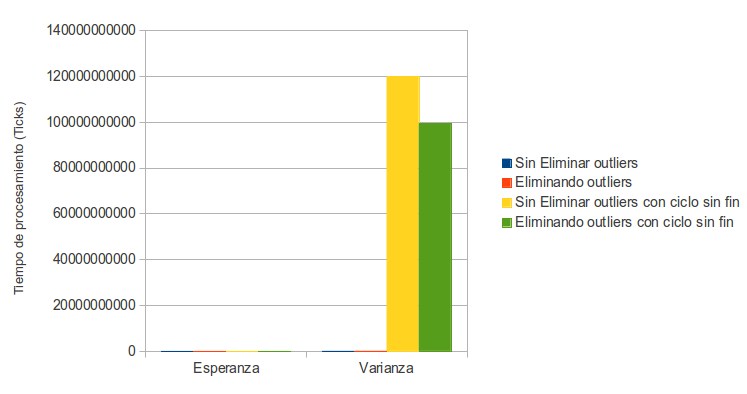
\includegraphics[width=\textwidth,height=\textheight,keepaspectratio
]{graficoasm.png}
\begin {flushleft}
\end{flushleft}
\vspace{0.4cm}
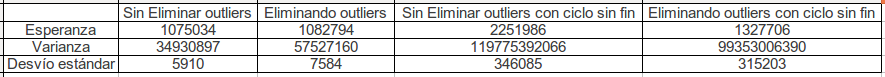
\includegraphics[width=\textwidth,height=\textheight,keepaspectratio
]{tablaASM.png}
\begin {flushleft}
\end{flushleft}
\newpage
En C: \newline
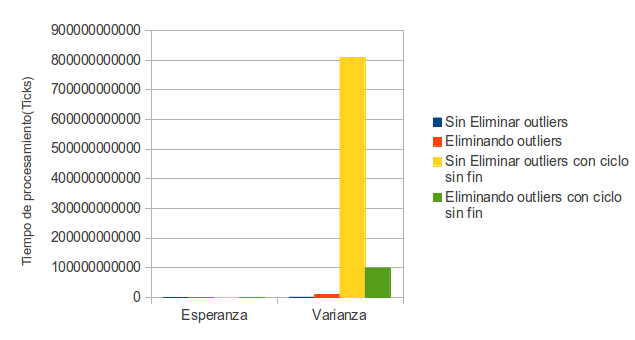
\includegraphics[width=\textwidth,height=\textheight,keepaspectratio
]{graficoC.png}
\begin {flushleft}
\end{flushleft}
\vspace{0.4cm}
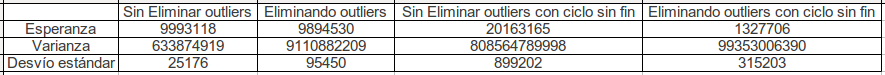
\includegraphics[width=\textwidth,height=\textheight,keepaspectratio
]{tablaC.png}
\begin {flushleft}
\end{flushleft}


Como podemos observar cuando corremos el ciclo sin fin la varianza aumenta, y cuando sacamos los ouliers la varianza disminuye.\newline
Esto se debe a que los resultados que obtenemos cuando corremos el ciclo sin fin tienen "picos altos y bajos muy marcados" y al eliminarlos la varianza baja notablemente.
\newpage

\subsection{Experimento 1.4 - secuencial vs. vecorial:}

\vspace{0.4cm}
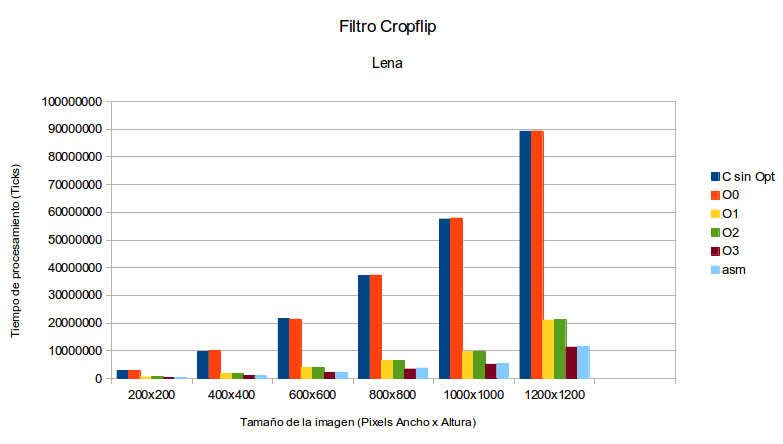
\includegraphics[width=\textwidth,height=\textheight,keepaspectratio
]{graficoOpt.png}
\begin {flushleft}
\end{flushleft}
Una tabla con la esperanza: \newline
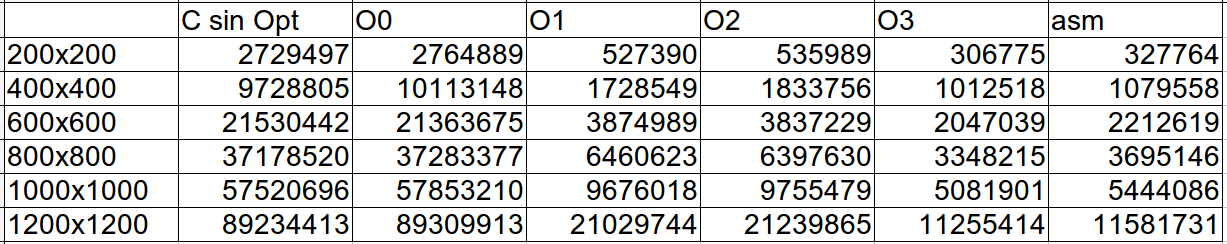
\includegraphics[width=\textwidth,height=\textheight,keepaspectratio
]{tablaEsperanzaOpt.png}
\begin {flushleft}
\end{flushleft}

Una tabla con el desvío estándar:\newline
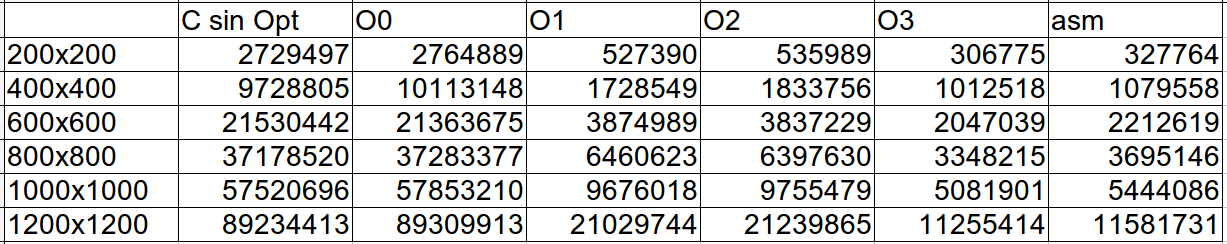
\includegraphics[width=\textwidth,height=\textheight,keepaspectratio
]{tablaEsperanzaOpt.png}
\begin {flushleft}
\end{flushleft}

Intuitivamente creíamos que ninguna optimización podría ganarle a la implementación de asm porque esta utiliza operaciones SIMD que permiten manejar más cantidad de datos en 1 operación, pero O3 le gana.
Esto es porque utiliza vectorización, y operaciones que tienen menor "costo" que las que usamos nosotros en asm.
La optimización O3 es lo suficientemente "inteligente" como para traducir el código c a asm usando SIMD, ganandole en tiempo de ejecución a nuestra implementación en asm.\newline
De todos modos la diferencia en performance es mínima. \newline
Se puede observar a simple vista que la implementación de c sin optimizaciones (o con O0) tiene una performance muy mala en comparación con la de asm y las optimizadas.
Como mencionamos en el experimento 1.1, el flag O1 optimiza el espacio, entonces la performance no se ve afectada prácticamente.
El flag O2 cambia intrucciones lentas por otras más rápidas, en este caso se ve que el tiempo de ejecución se redujo a más de la mitad al igual que con el flag O2.
Con el flag no hay diferencia porque solo acota el tiempo de compilación.
Y finalmente el flag O3 reduce drásticamente el tiempo de ejecución. 
\newline


\subsection{Experimento 1.5 - cpu vs. bus de memoria:}

Intuitivamente los accesos a memoria son mas caros que las operaciones lógicas y las aritméticas, veamos que sucede con los gráficos.
\newline
Usando add, subb, shl shr con rax (porque no está ocupado por el código) para las instrucciones aritméticas/ lógicas
y lecturas y escrituras en las matrices de entrada y salida.\newline
Usando la pila también cumplía el objetivo de agregar "instrucciones de memoria" pero accediendo a disco es mucho más evidente el costo.\newline
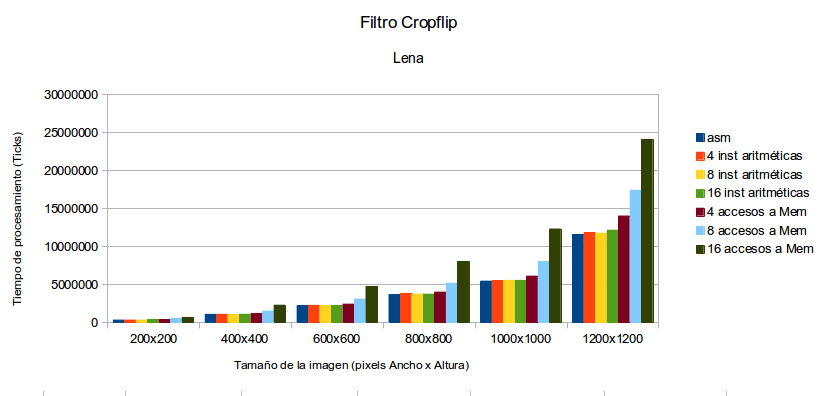
\includegraphics[width=\textwidth,height=\textheight,keepaspectratio
]{graficoMenVsArit.png}
\begin {flushleft}
\end{flushleft}

Una tabla con la esperanza: \newline
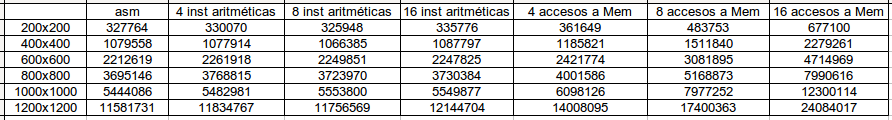
\includegraphics[width=\textwidth,height=\textheight,keepaspectratio
]{tablaMenVsArit.png}
\begin {flushleft}
\end{flushleft}

Una tabla con el desvío estándar:\newline
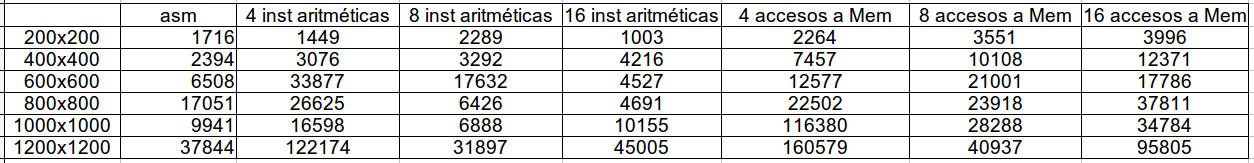
\includegraphics[width=\textwidth,height=\textheight,keepaspectratio
]{tablaVarianzaMenvscpu.png}
\begin {flushleft}
\end{flushleft}
Como vemos en el gráfico cuando aumentamos la cantidad de accesos a memoria, el tiempo de ejecución se ve afectado negativamente, es mucho más lento.
En cambio cuando agregamos instrucciones aritmeticas el cambio en performance es mínimo.
Con lo cual podemos concuir que los accesos a memoria son el factor que limita la performance.



\subsection{Experimento 2.1:}

\subsection{Secuencial vs vectorial:}

En la $figura$ $Sierpinski\_1$ se grafico el tiempo de procesamiento para el filtro Sierpinski en lenguaje ASM y C, ademas para este último se lo calculo  sin activar flags de optimización y luego con los flags -O0, -O1. -O2, -O3. Por cada tamaño de la imagen se generaron 10 mediciones de un total de 1000 tiempos cada una. Luego, se procedio a eliminar los outliers, calcular el promedio de cada medición y un promedio de en general de estos. Que es el valor graficado. 

\vspace{1cm}
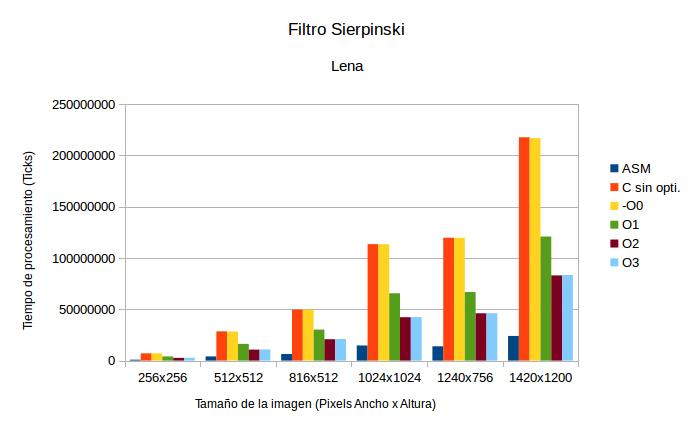
\includegraphics[width=\textwidth,height=\textheight,keepaspectratio
]{sierppri.jpg}
\textit{figura Sierpinski\_1: Se muestran las diferencias en el tiempo de procesamiento de cada imagen según el lenguaje utilizado y el uso o no de flags de optimización} \newline \newline


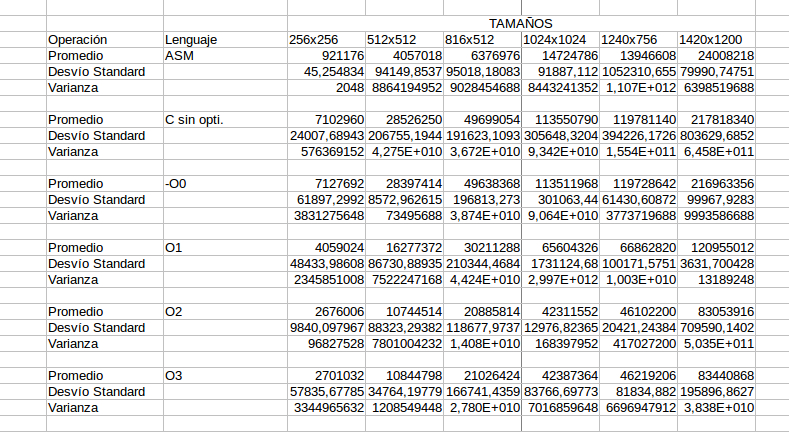
\includegraphics[width=\textwidth,height=\textheight,keepaspectratio
]{flags.jpg}
\textit{Se detallan los valores promedios graficados en la figura Sierpinski\_1, ademas de la varianza y el desvio Standard de cada una de las imagenes}\newline \newline

En el gráfico se puede comprobar la eficacia de utilizar lenguaje ASM, en vez de C. Pese a que en este último se utilicen flags de optimizacón esta gran diferencia es generada en mayor parte por el tipo de instrucciones disponible en lenguaje ASM, que son las intrucciones SSE. Las cuales me permiten manipular hasta 16 bytes de datos por acceso a memoria. En cambio en C solo puedo trabajar de a 4 bytes. Es decir, un pixel. Como se debe escribir sobre toda la imagen destino. Y en ambos lenguajes se emplean ciclos para recorrerla, la cantidad de iteraciones que debo hacer en C son 4 veces más que para ASM, ya que en este por cada iteración se trabaja con 4 pixels. Esto ya representa una ventaja para el código ASM. Ademas, con solo un acceso a memoria puedo leer 4 pixels. y con otro acceso puedo escribir estos 4. En cambio en C por cada acceso a memoria solo puedo leer un solo pixel. No solo estoy aumentando la cantidad de iteraciones en este código sino que estoy aumentando los accesos a memoria. Si bien el código en ASM requiere de mas instrucciones aritmeticas, o logicas. El limitante en el rendimiento esta dado por las intrucciones de acceso a memoria (hecho que se explica en el $experimento$ $2.1$ $cpu$ $vs.$ $bus$ $de$ $memoria$). Por lo que utilizar el codigo en lenguaje ASM es mucho mas eficiente. Sin embargo a la hora de utilizar el lenguaje C pueden ocurrir diferencia en el tiempo de procesamiento según se utilicen o no flags. En el gráfico se observa que no utilizar flags o bien utilizar -O0, que deshabilita todas las optimizaciones, es lo menos eficiente. El mayor tiempo corresponde a estos dos casos. Al habilitar el flag -01 este se encarga de optimizar en espacio. Lo que reduce casi a la mitad el tiempo de procesamiento. Lo que puede ocurrir es que el tiempo se reduzca al intentar optimizar el espacio o la velocidad, generalmente esta última a traves del reeemplazo de instrucciones por otras más rápidas. En este caso el tiempo se reduce por este último hecho. Mejorar la velocidad influye mas en  este filtro que el espacio. Hecho realizado por los flags -02 y -O3. Posiblemente  utilizar estos flags en este filtro sea mejor ya que los pixels en en el mismo estan sujetos a varias operaciones matemáticas(las mismas son descriptas en la parte de $Desarrollo$ $filtro$ $Sierpinski$) y se esten reemplazando las instrucciones elejidas por otras con mejor rendimiento.


\subsection{Experimento 2.1:}


\subsection*{cpu vs. bus de memoria:}

Para determinar cual es el mayor limitante a la perfomance del Filtro Sierpinski es su versión de ASM. Se procedio a modificar el código general agregando intrucciones que requieran acceso a memoria y otras que no (aritmeticas) .Para esto se hicieron un total de 6 modificaciones. 3 corresponden a agregar instrucciones, al ciclo que recorre la imagen, aritmeticas. Y las otras tres a agregar instrucciones que realizan accesos a memoria. Para cada caso se agregaron 4, 8 y luego 16 instrucciones. Una vez modificados los archivos. Se calcularon 10 mediciones, donde cada una de estas tiene un total de 1000 tiempos. Se calculo el prmedio de cada una y un promedio en general. Para todos estos casos los resultados son los que se observan en la $figura$ $Sierpinski\_2$ 

\vspace{1cm}
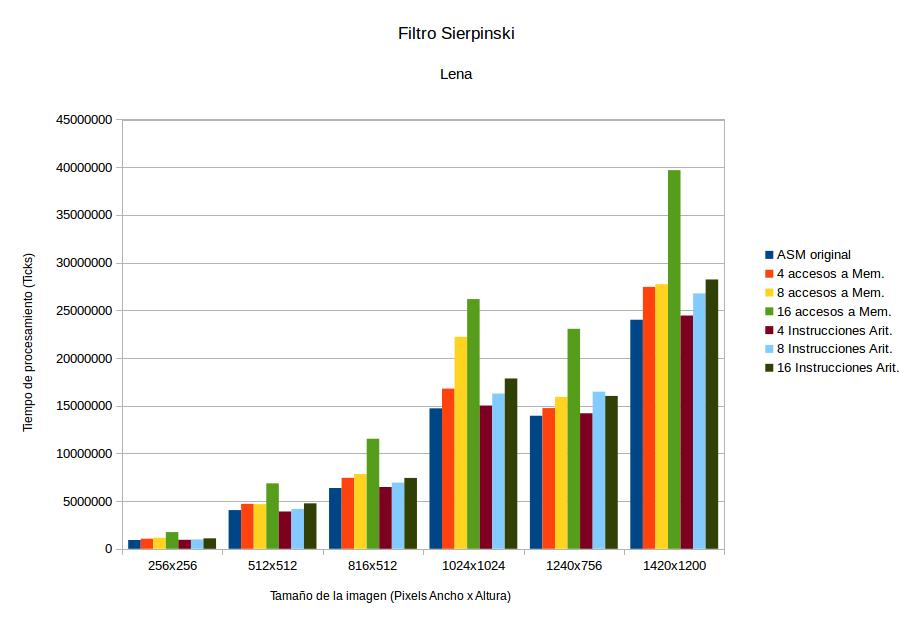
\includegraphics[width=\textwidth,height=\textheight,keepaspectratio
]{sierpseg.jpg}
\textit{figura Sierpinski\_2: Se muestran las diferencias en el tiempo de procesamiento de cada imagen en lenguaje ASM, donde se fueron agregando distintas modificaciones al código original} \newline \newline

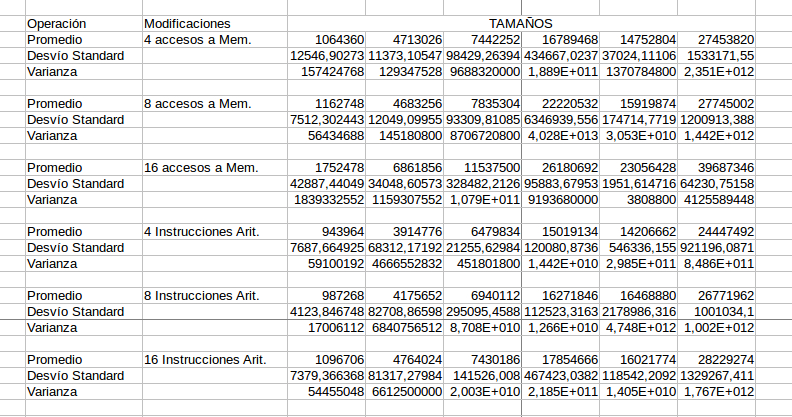
\includegraphics[width=\textwidth,height=\textheight,keepaspectratio
]{modifi.jpg}\textit{Se detallan los valores promedios graficados en la figura Sierpinski\_2, ademas de la varianza y el desvio Standard de cada una de las imagenes}\newline \newline

Las intrucciones aritmeticas que se agregaron fueron:\newline
Caso: 4 nuevas instrucciones aritméticas 
add rax, rdx \newline
add rax, rcx\newline
sub rax, r8\newline
sub rax, r9\newline
\textit{rax es el único registro que no se utiliza en el código original. Por lo que se procedio a modificar este para evitar alterar a los demas y por ende el resultado del filtro. rdx representa al contador de filas, rcx al de columnas y r8 y r9 a src\_row\_size y dst\_row\_size respectivamente.}\newline
8 nuevas instrucciones aritméticas \newline	
inc rax\newline
inc rax\newline
shr rax, 2\newline
shl rax, 2\newline
\textit{A las instrucciones que ya habia para el caso 4 instrucciones aritmeticas, se le incorporaron estas nuevas.}\newline
16 nuevas instrucciones aritméticas \newline
shr rax, 2\newline
dec rax\newline
dec rax\newline
lea rax, [r8*2]\newline
lea rax, [r9*2]\newline
shl rax, 2\newline
shl rax, 2\newline
add rax, rax\newline
\textit{Se agregaron estas 8 intrucciones al caso anterior}\newline
Las instrucciones de accesos a memorias fueron:\newline
Caso: 4 nuevas instrucciones de acceso a memoria\newline
movdqu xmm4, [fuente + r12]\newline
movdqu [destino], xmm4\newline
movdqu xmm4, [destino + r12]\newline
movdqu [fuente], xmm4\newline
\textit{fuente representa el puntero al inicio de la matriz fuente, y destino al inicio de la matriz destino, r12 actua como offset para desplazarme por las columnas. El mismo se va modificando en cada iteración de esta forma evito que se cachen espacios de memoria. Lo que reducidia el tiempo de acceso.}\newline
8 nuevas instrucciones de acceso a memoria\newline	
mov eax, ebx\newline
movdqu xmm4, [fuente + rax]\newline
movdqu [destino +rax ], xmm4\newline
inc rax	\newline
movdqu xmm4, [destino + rax ]\newline
movdqu [fuente + rax], xmm4\newline
\textit{ A las intrucciones del caso anterior se le agregaron estas 4 nuevas, en este caso ebx es el contador de filas. Como tambien va variando en cada iteracion siempre voy a leer de un nuevo espacio de memoria evitando cachearla.}\newline
16 nuevas instrucciones de acceso a memoria\newline
inc rax\newline
movdqu xmm4, [fuente + rax]\newline
movdqu [destino +rax ], xmm4	\newline
movdqu xmm4, [destino + rbx]\newline
movdqu [fuente + rbx], xmm4\newline
add rax, rbx	\newline
movdqu xmm4, [fuente + rax]\newline
movdqu [destino +r12 ], xmm4	\newline
movdqu xmm4, [destino + r12]\newline
movdqu [fuente + rax], xmm4\newline
\textit{Por último se agregaron estas 8 instrucciones al caso anterior. Las mismas realizan lo mismo que las otras pero en espacio diferentes de memoria. Leen los datos de una determinada sección de la imagen fuente y los escriben en otra de la imagen destino}\newline
Como se puede observar en la $figura$ $Sierpinski\_2$. El mayor limitante son las intrucciones de acceso a memoria. Ya que el acceder cada vez más a memoria aumenta notablemente tiempo de procesamiento. Se puede ver que existe un equilibrio en cuanto al tiempo de procesamiento entre el caso de agregar operaciones aritmeticas y las de acceso a memoria. Solo cuando la cantidad de instrucciones de las primeras son en mayor cantidad que las segundas. Si se agrega la misma cantidad de instrucciones entonces el tiempo de procesamiento va a ser mayor para aquellas que requieran acceder a memoria. En conclusión la perfomance esta limitada por los accesos a memoria.  
\newpage
\subsection{Experimento 3.1 - saltos condicionales}

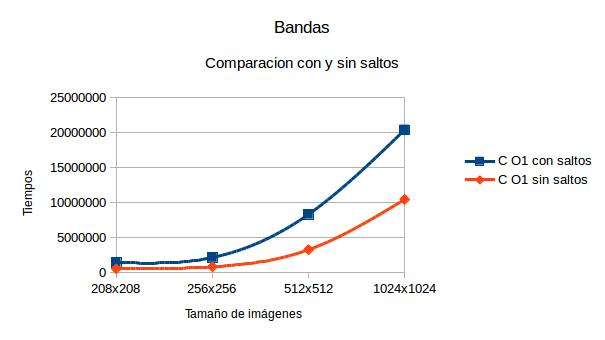
\includegraphics[height=6cm]{imagenes/bandasCsaltos.jpg}

% ******************************************************************************


\vspace*{0.3cm} \noindent
\subsection{Experimento 3.2 - secuencial vs. vectorial}

En los testeos que hicimos con las im\'agenes y sus distintos tamaños, notamos como los outliers y la varianza aumenta a medida que se utiliza una im\'agen m\'as grande.
Adem\'as de \'esto, en los graficos puede observarse la notable diferencia de tiempos entre las versiones y las optimizaciones del compilador.

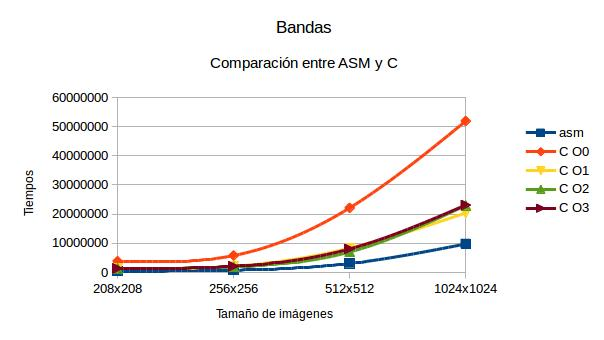
\includegraphics[height=6cm]{imagenes/bandasAsmC.jpg}


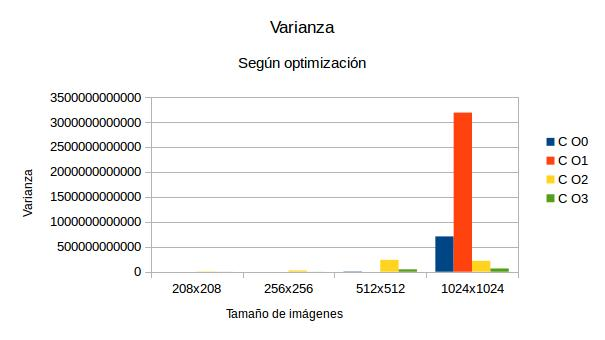
\includegraphics[height=6cm]{imagenes/bandasVarianza.jpg}

\subsection{Experimento 4.1:}

\subsection{secuencial vs vectorial:}

En la $figura$ $MBlur\_1$ se muestra la perfomance, medida en ticks, para la imagen provista (Lena). Realizando una comparacion entre la perfomance obtenida al ejecutar el filtro en lenguaje ASM y C, este último en 5 casos distintos, sin flags de optimización, y con los flags -O0, -O1, -O2, -O3. Se repitio por cada tamaño de la imagen 10 mediciones de un total de 1000 tiempos cada una. Luego, se procedio a eliminar los outliers, calcular el promedio de cada medición y un promedio de en general de estos. Que es el valor graficado. En el grafico se puede apreciar la superioridad del procesamiento en ASM contra el de C, incluso con los flags de optimización.
Esto se debe al uso de las instrucciones SSE, que permiten leer
en un solo acceso a memoria, 16 bytes de datos; mientras que una operación en C permite a lo sumo la lectura de 4 bytes por acceso a memoria, un byte por cada color del struct $’bgra\_t’$ mostrado a continuación 
$typedef$ $struct$ $bgra\_t$ $\{$\newline
	$unsigned$ $char$ $b,$ $g,$ $r,$ $a;$ \newline
$\}$ $\_\_attribute\_\_((packed))$ $bgra\_t;$ \newline

\vspace{1cm}
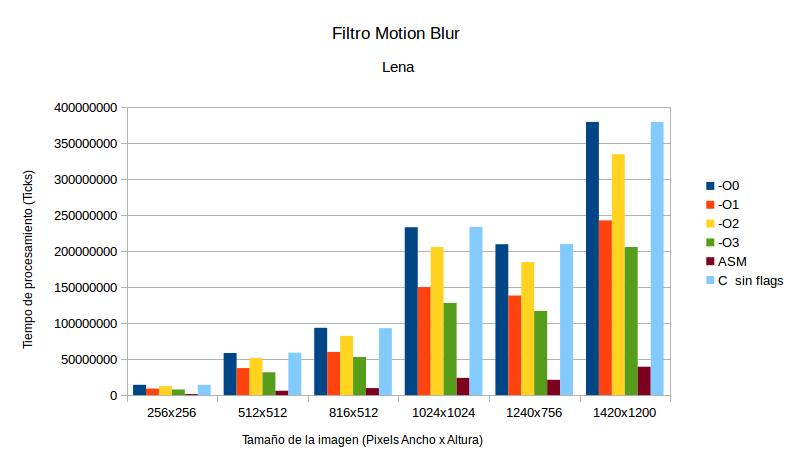
\includegraphics[width=\textwidth,height=\textheight,keepaspectratio
]{mblur.jpg}
\textit{figura MBlur\_1: Se muestra las diferencias en el tiempo de procesamiento de cada imagen según el lenguaje utilizado y el uso o no de flags de optimización} \newline \newline

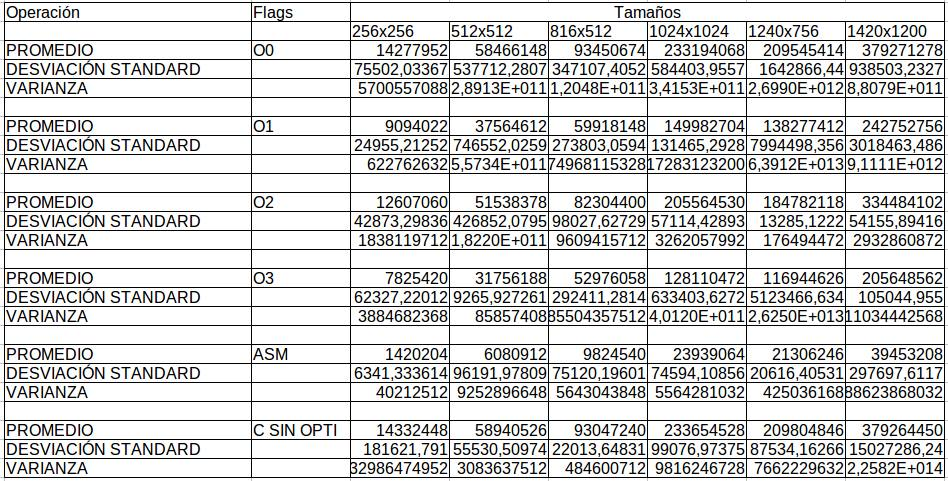
\includegraphics[width=\textwidth,height=\textheight,keepaspectratio
]{valoresmblur.jpg}
\textit{Se detallan los valores promedios graficados en la figura Mblur, ademas de la varianza y el desvio Standard de cada una de las imagenes}\newline \newline


Esto me va a permitir recorrer la imagen y escrbir los resultados en la matriz destino en una cantidad de iteraciones menor que las que utilizadas en C. Aun con los flags de optimización la perfomance de ASM es mucho menor. Ya que algunas de las acciones que realizan los flags son eliminación del código muerto, o no pasar todos los parametros por la pila. Lo cual reduce el tiempo de procesamiento pero, la cantidad de pixels analizado sigue siendo de a uno. Y como particularmente este filtro por cada posición a escribir necesita del acceso a memoria de otros 5 pixels. Cada vez que en C quiero escribir un valor leo 5 veces de memoria. Mientras que en ASM si bien leo la misma cantidad por iteracion del mencionado $ciclo$ $principal$, esas lecturas me permiten escribir luego 16 bytes de datos en un solo acceso a memoria. Es decir un ciclo en ASM equivale a 20 accesos a memoria en el lenguaje C. Por lo que no solo la perfomance se ve afectada por la cantidad de iteraciones que realiza cada lenguaje para escribir en toda la matriz destino. Sino que nos estamos ahorrando accesos a memoria y como se ha visto  en otros filtros por ejemplo en la $experimento$ $2.1$ el mayor limitante a la perfomance esta dado por los accesos a memoria que se realizan. Y no tanto por las instrucciones que no requiren accesos. Ya que a diferencia del lenguaje en C, el código es ASM utiliza muchas mas intrucciones logicas, aritmeticas. Por lo que se puede concluir que el lenguaje ASM en mas óptimo que el de C. No solo podemos concluir esto a partir de las mediciones realizadas, sino que según que flags utilicemos, la perfomance del código en C tambien va a variar. Como se puede obervar la perfomance sin flags de optimizacón es mayor que cuando se los usa. Ya que cada uno de los flags trata de realizar una mejora especifica en el código. Esta variación se ve para todos los flags menos para el -O0 ya que este en realidad deshabilita todas las optimizaciones entonces tiene sentido que el tiempo de ejecución sea el mismo que el que no tiene los flags activado. El flag -O1    
optimiza en espacio, si hay optimizaciones que aumentan el tamaño tambien las va a omitir. En el gráfico se puede observar que el realizar esto influye notablemente en el procesamiento de la imagen. el siguiente flag -O2 optimiza en velocidad se reemplazan instrucciones que demoran mas por otras que no lo hacen. En este caso pese a que es mejor que sin ejecutar el flag. usando -O1 se obtiene una mejor perfomance. Por lo que uno de los mayores problemas en cuanto al rendimiento esta dado por el tamaño utilizado. Finalmente el flag -03 realiza una mejora agresiva sobre la velocidad es decir, utliza instrucciones de mas alto nivel que para -O2. Y utilizar este es mejor que para el -O1. Entonces si bien ahorrar espacio puede ser mejor que el reemplazar instrucciones por otras. Si se realizan los intercambios correctos puede llegar a ser mas óptimo. En conclusion, en este caso, el lenguaje ASM es mas efectivo, en cuanto a perfomance, que el lenguaje C. Pero este último tambien puede variar segun los flags utilizados, usar -03 fue lo mas óptimo. 


\newpage

{\noindent \Huge Conclusiones:}


Podemos concluir varias cosas, primero escribir código en C es cómodo e intuitivo. En cambio, escribirlo en ASM no es nada trivial, encontrar errores es difícil, hay que tener conciencia de como se maneja lo que estamos leyendo en memoria y donde se escribe.

Sin embargo se puede ver claramente en las experimentaciones  que el tiempo de ejecución de las implementaciones en asm es mucho mejor que las de c.
Lo cual era esperable dado que procesamos muchos datos a la vez y solo hacemos accesos a memoria dentro de
los ciclos para cargar los pixels de la imagen fuente y para escribirlos luego de procesarlos.

En cuanto al compilador se puede observar que cuando no tiene optimizaciones los algoritmos corren lento(en comparación con asm), y cuando se agregan los flags de optimizaciones los algoritmos corren a una diferencia más que notable. \newline
Incluso en cropflip el flag O3 supera mínimamente en performance a la implementación en asm, lo que nos llamó mucho la atención. 

\newpage

{\noindent \Huge Anexo:}
\newline \newline

Todas las mediciones, junto con su promedio, varianza y desvio Standard se encuentran en la carpeta $Anexo$. Ademas se incluyen los archivos modificados para la experimentación cpu vs bus de memoria.


\end{document}
